\section{Coordinate System} \label{sec:coordinate_system}

\subsection{Body-Fixed Coordinate System} \label{subsec:body_fixed_coordinate_system}

To further refine the vehicle's representation, we introduce the body-fixed coordinate system, which is attached to the moving reference position of
the vehicle within the global coordinate system.
The first axis of the body-fixed coordinate system aligns with the vehicle's longitudinal orientation and is denoted by the unit vector $e_{b,x}$.
The second axis is orthogonal to the first and is denoted by $e_{b,y}$.
This coordinate system simplifies modeling control inputs and forces acting on the vehicle.

\subsection{Frenet Frame Representation} \label{subsec:frenet_frame}

In our previous models, vehicle positions and orientations were represented using a global Cartesian coordinate system.
While this approach is effective for modeling vehicle dynamics, it becomes cumbersome when incorporating road topology constraints.

Since road topology is typically known in advance, we can leverage this knowledge to define a coordinate system that simplifies constraint modeling.
The Frenet frame provides a more intuitive way to describe vehicle motion relative to a reference path, resulting in a more structured and often
convex constraint representation.

The Frenet frame consists of two coordinates, $(s, n)$, where $s$ represents the arc-length position along the reference curve, and $n$ denotes the
orthogonal deviation from it.
This transformation allows constraints to be naturally aligned with the road structure, simplifying feasibility checks and trajectory optimization.

\begin{figure}[h]
	\centering
	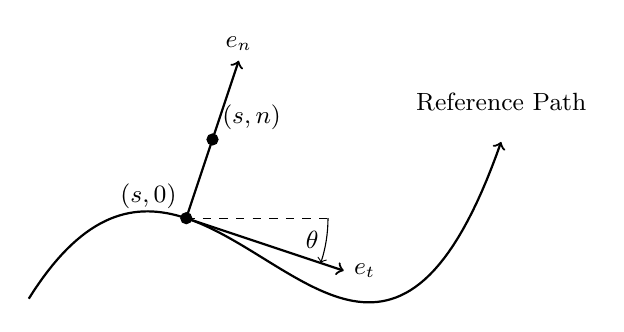
\begin{tikzpicture}
		% Draw the reference path (a smooth curve)
		\draw[->, thick, domain=2:8, samples=100] plot (\x, {-5 + 4.466667*(\x) - 0.7444444*(\x)^2 - 0.005555556*(\x)^3 + 0.005555556*(\x)^4});

		% Label the reference path
		\node[black] at (8,3.5) {\small Reference Path};

		% Point on the reference path
		\filldraw[black] (4,2.022224352) circle (2pt);
		\node[above left] at (4,2.022224352) {\small $(s, 0)$};

		% Draw tangent and normal vectors
		\draw[->, thick] (4,2.022224352) -- (6,1.3555515519999999) node[right] {\small $e_t$};
		\draw[->, thick] (4,2.022224352) -- (4.6666728,4.022224352) node[above] {\small $e_n$};

		% Theta angle
		\draw[dashed] (4,2.022224352) -- (5.8,2.022224352);
		\draw[->] (5.8,2.022224352) arc (0:-18.43510695912798:1.8);
		\node at (5.6,1.75) {\small $\theta$};

		% Off-path point (s, n)
		\filldraw[black] (4.333336399999999,3.022224352) circle (2pt);
		\node[above right] at (4.333336399999999,3.022224352) {\small $(s, n)$};
	\end{tikzpicture}
	\caption{Frenet Frame Representation}
	\label{fig:frenet_frame}
\end{figure}

Let $\theta(s)$ denote the angle between the tangent vector at position $s$ along the reference path and the $x$-axis of a global fixed coordinate
system.
If the global position of the reference path at the starting point $s_{\min}$ is known, the global coordinates of any point along the reference path can be determined using:

\begin{align}
	p_x(s) & = \int_{s_{\min}}^{s} \cos(\theta(\sigma)) d\sigma + p_x(s_{\min}), \\
	p_y(s) & = \int_{s_{\min}}^{s} \sin(\theta(\sigma)) d\sigma + p_y(s_{\min}).
\end{align}

The reference path is aligned with the road, allowing the vehicle's position to be described within this Frenet frame.
In the following section, we will transition the point mass model's dynamics into this coordinate system.

